%&LaTeX
% !TEX encoding = UTF-8 Unicode
\documentclass{article}
\usepackage{listings}

\lstset{
	language = Java,
         basicstyle=\footnotesize\ttfamily,
         numberstyle=\tiny,
         numbersep=5pt,       
         tabsize=2,                  
         extendedchars=true,    
         breaklines=true,            
         keywordstyle=\color{red},
%    		frame=b,         
         stringstyle=\color{white}\ttfamily, 
         showspaces=false,           
         showtabs=false,             
         xleftmargin=17pt,
         framexleftmargin=17pt,
         framexrightmargin=5pt,
         framexbottommargin=4pt,
         showstringspaces=false   
 }
 \lstloadlanguages{Java}

\usepackage{caption}
\DeclareCaptionFont{white}{\color{white}}
\DeclareCaptionFormat{listing}{\colorbox[cmyk]{0.43, 0.35, 0.35,0.01}{\parbox{\textwidth}{\hspace{15pt}#1#2#3}}}
\captionsetup[lstlisting]{format=listing,labelfont=white,textfont=white, singlelinecheck=false, margin=0pt, font={bf,footnotesize}}

\usepackage[utf8]{inputenc}
\usepackage[francais]{babel}
\usepackage[T1]{fontenc}
\usepackage{textcomp}
\usepackage[colorlinks=true, linkcolor=black, urlcolor = blue]{hyperref}

\usepackage{graphicx}
\usepackage{ulem}
\usepackage{color}
\usepackage[top=2.5cm,bottom=3cm,left=3cm,right=3cm]{geometry}


\definecolor{color01}{rgb}{0.00,0.00,0.00}
\definecolor{color02}{rgb}{0.40,0.40,0.40}
\definecolor{color03}{rgb}{0.07,0.33,0.80}


\title{\Huge{AGETAC\\
Aide à la GEstion TACtique\\}
\huge{{\color{color02} \textit{Document de développement}}}}

\date{Mai 2012}
\author{Projet Agetac - Université de Rennes 1\\
Encadré par Noël Plouzeau}



\begin{document}
\vspace{0.5in}
\maketitle
\newpage
$~$
\vspace{0.5in}
\tableofcontents
\newpage
\section{Introduction}

\subsection{Présentation du document}

Le présent document s'adresse aux futurs développeurs ou chargés de maintenance d’Agetac. Il présente de manière détaillée la procédure à suivre pour pouvoir récupérer les fichiers sources du projet, explique brièvement l'architecture des fichiers et enfin il montre comment modifier ou ajouter des fonctionnalités.

\subsection{GitHub}

Dans tout projet conséquent, la gestion des documents, des versions et des mises à jour posent souvent problème. Dès la mise en place du projet Agetac, nous avons choisi d'utiliser GitHub, un service qui permet d'héberger des projets libres pour gérer les sources et les documents relatifs au projet.

Tous les documents, sources, et exécutables sont téléchargeables à cette adresse :\\ \url{https://github.com/Agetac}

\section{Installer l'environnement}


\subsection{Java}

Le projet a été exclusivement développé dans le langage Java. Le choix de ce langage a été

fait depuis le départ pour des raisons de portabilité. Java est également un langage libre, dont la communauté est très active sur Internet.


\subsection{Android}

Le projet a été développé pour fonctionner sur tablette tactile Android utilisant la version 3.0. 


\subsection{Les librairies utilisées}

\subsubsection{Jackson}

Nous avons intégré à Restlet l'extension Jackson pour la communication entre le serveur et les tablettes. Jackson est une librairie très rapide qui permet de sérialiser des objets Java en JSON (JavaScript Object Notation) de façon standard, et inversement de convertir du JSON en objets Java.

\subsubsection{DataNucleus}

Il s’agit d’un projet open-source qui offre des librairies permettant l'accès aux données utilisant des API standards pour un grand nombre de banques de données. Nous utilisons donc DataNucleus pour gérer notre modèle de persistance qui est JDO (Java Data Object) avec notre système de gestion de données.

\subsubsection{HSQLDB}

Cette librairie nous permet de manipuler notre système de gestion de bases de données     relationnelles (RDBMS - Relational DataBase Management System ) Java du même nom.    

\subsubsection{ModelMapper}

ModelMapper est un framework de mapping d'objet intelligent qui élimine le besoin de mapper les objets manuellement les uns aux autres dans la persistance.    

\subsubsection{HttpClient et HttpCore de Apache}

Ces librairies nous offrent un support plus robuste du protocole HTTP que les packages Java basiques.

Avec le client HTTP par défaut de Restlet, nous avions des problèmes de communication entre la tablette cliente et le serveur. En effet, il semble que ni Android ni le client HTTP de Restlet ne pouvaient gérer correctement l’encodage de transfert qui est activé par défaut dans le client HTTP de Restlet et impossible à désactiver.

\section{Structure du projet / Rôle des classes}

\subsection{Model}

\subsubsection{Diagramme de classe}

\begin{figure}[htbp]
\begin{center}
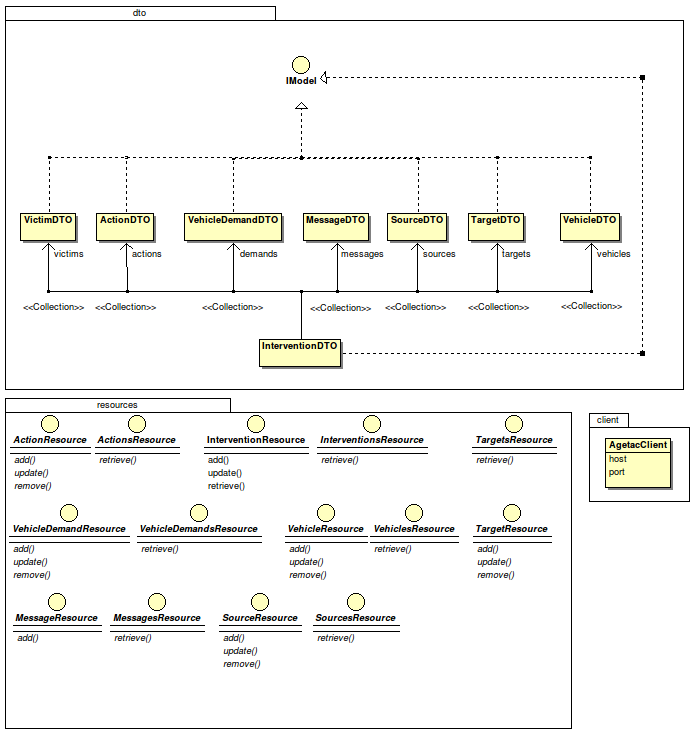
\includegraphics[width=400pt]{doc_dev-fig001.png}
\caption{Diagramme de classe pour Model}
\label{1}
\end{center}
\end{figure}

\newpage

\subsubsection{Package resources}

Contient toutes les interfaces des ressources ainsi que les classes du package “resources” que le serveur doit implémenter.

\subsubsection{Package observer}

Contient la classe \textbf{MyObservable} qui étend \textbf{java.util.Observable} et qui rend publique la méthode textbf{setChanged()}.

L'intérêt du pattern Observer est de prévenir les classes observatrices via un « signal » d'un changement sur les classes observées afin d'effectuer une action relative à ce changement.

Ce pattern est utilisé principalement dans le client pour mettre à jour les données.

\subsubsection{Package dto}

Ces classes représentent des ressources, « \textbf{typeDTO.java} », qui sont amenées à être échangées entre la tablette cliente et le serveur. Ce sont ces objets qui transitent sur le réseau.

Nous ne transférons pas les entités ORM (Object-Relational Mapping) car, à moins d’être très attentif, il y a le risque de récupérer plus d’informations que voulu de l’arbre de données de l’objet si Jackson sérialise une entité ORM (pour la faire passer à travers le réseau).

\subsubsection{Package client}

« \textbf{AgetacClient.java} » est une classe “protocolaire” connaissant les opérations GET, POST, PUT, DELETE à effectuer sur les différentes ressources (telle une demande de véhicule ou l'ajout d'une victime). Les fonctions associées effectuent les opérations REST correspondantes : elles créent une ressource \textbf{typeDTO}, à laquelle est associée une URI (Uniform Resource Identifier), qui sera envoyée au serveur.

L’idée était d’avoir une (dé)sérialisation JSON complètement transparente en utilisant une extension Restlet de conversion automatique. Par exemple, en utilisant cette méthode, le client peut exécuter le code suivant pour récupérer un véhicule :


\begin{lstlisting}
ClientResource clientResource = new ClientResource(someurl);
try {
    VehicleResource vehicleResource = clientResource.wrap(VehicleResource.class);
    return  vehicleResource.retrieve();
} finally {
    clientResource.release();
}
\end{lstlisting}


Cependant, utiliser cette méthode pour (dé)sérialiser des collections d’objets ne fonctionne pas (correctement). Par exemple, une \textbf{Collection<InterventionDTO>} sur le serveur convertie en JSON et transmise via Restlet devient une \textbf{Collection<LinkedHashMap>} sur le client.

La représentation \textbf{JacksonRepresentation} utilise un \textbf{Mapper} pour faire la conversion mais les types paramétrés ne sont pas conservés donc le type de retour devient une Collection simple. A la réception, Jackson fait de son mieux pour recréer l’objet mais un objet sérialisé en JSON ressemble à une \textbf{Map}, c’est donc ce qu’il choisit.

Pour éviter cette perte d’information de type, nous avons utilisé Jackson directement plutôt que la conversion automatique de Restlet. Ainsi, nous pouvons passer des informations complètes sur les types. Par exemple, la méthode pour récupérer une liste d’interventions est implémentée de la façon suivante :

\begin{lstlisting}
try {
    Representation repr = clientResource.get();
    TypeReference<Collection<InterventionDTO>> tr = new TypeReference<Collection<InterventionDTO>>() {};
    ObjectMapper mapper = new ObjectMapper();
    Collection<InterventionDTO> col = null;
    col = mapper.readValue(repr.getStream(), tr);
    return col;
} catch (Exception e) {
    e.printStackTrace();
} finally {
    clientResource.release();
}
\end{lstlisting}


\subsection{Client}


\subsubsection{Package controller}
\begin{figure}[htbp]
\begin{center}
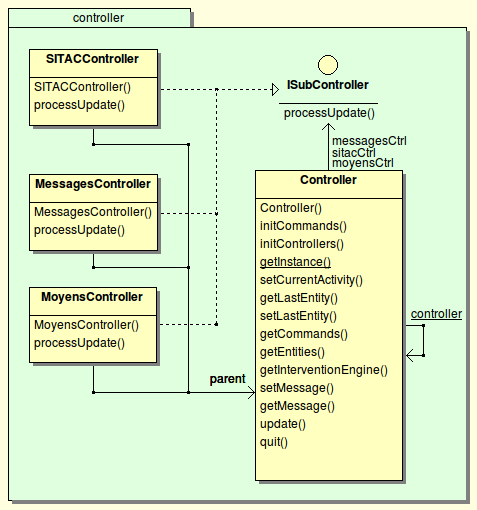
\includegraphics[width=350pt]{doc_dev-fig002.png}
\caption{Diagramme de classe du package controlleur.}
\end{center}
\end{figure}


Le \textbf{Controller} est en relation avec les différentes \textbf{XXXActivity} et le moteur de l’application.

C’est un singleton qui observe les changements des différentes Activity et qui appelle en conséquence le contrôleur associé à l'activité.

Le contrôleur observe aussi le moteur \textbf{InterventionEngine}. Lorsque celui-ci se met à jour, le contrôleur se charge d’appeler la méthode \textbf{update()} propre à l'activité de type \textbf{ITabActivity} courante.

Chaque sous-contrôleur \textbf{ISubController} correspond à une \textbf{ITabActivity} et sait comment traiter les informations en fonction de l’état de la variable de type \textbf{ActionFlag}.
\newpage

\subsubsection{Package activity}
\begin{figure}[htbp]
\begin{center}
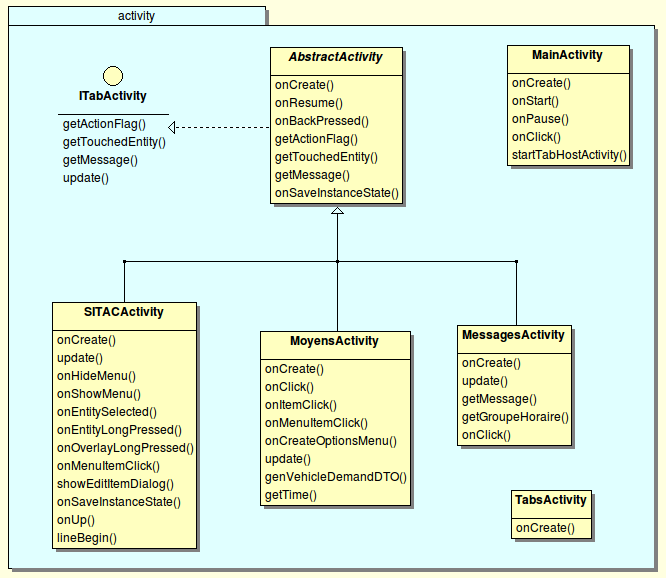
\includegraphics[height=433pt]{doc_dev-fig003.png}
\caption{Diagramme de classe du package activity.}
\end{center}
\end{figure}

Les activités forment l’interface graphique de l’application. Elles jouent aussi le rôle de “listener” en réagissant aux interactions de l’utilisateur. Aussi définissent-elles un \textbf{ActionFlag} approprié pour l’action en cours (ajout, suppression, update, …), ainsi qu’une \textbf{IEntity} courante (touchedEntity). Enfin, elles notifient à leur observateur quand leur état a changé.

\newpage
\subsubsection{Package fragment}
\begin{figure}[htbp]
\begin{center}
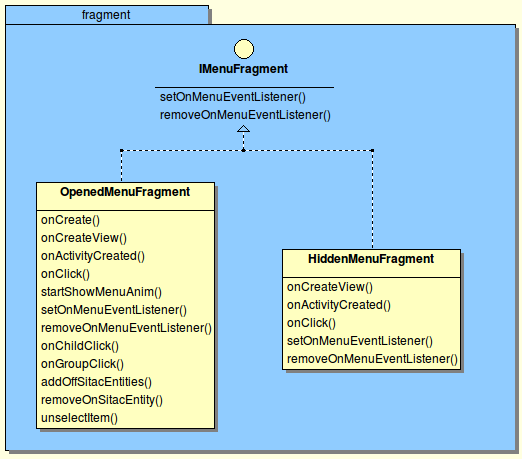
\includegraphics[width=391pt, height=344pt]{doc_dev-fig004.png}
\caption{Diagramme de classe du package fragment.}
\end{center}
\end{figure}

Les \textbf{IMenuFragment} sont des menus affichés dans l’onglet SITAC. On a deux menus :
\begin{itemize}
\item OpenedMenuFragment : menu ouvert sur la SITAC
\item HiddenMenuFragment : menu fermé sur la SITAC
\end{itemize}
Les menus sont capables de notifier les interactions de l’utilisateur via l’interface \textbf{IOnMenuEventListener}. Si une classe hérite de cette interface et s’enregistre comme “listener” d’un \textbf{IMenuFragment}, alors elle recevra des events en fonction des actions faites sur le menu.

\newpage
\begin{figure}[htbp]
\begin{center}
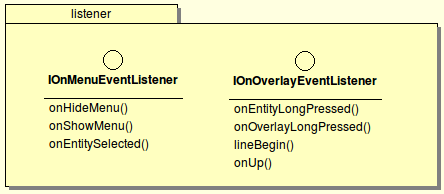
\includegraphics[width=260pt]{doc_dev-fig005.png}
\caption{Diagramme du package listener}
\end{center}
\end{figure}

\begin{figure}[hbtp]
\begin{center}
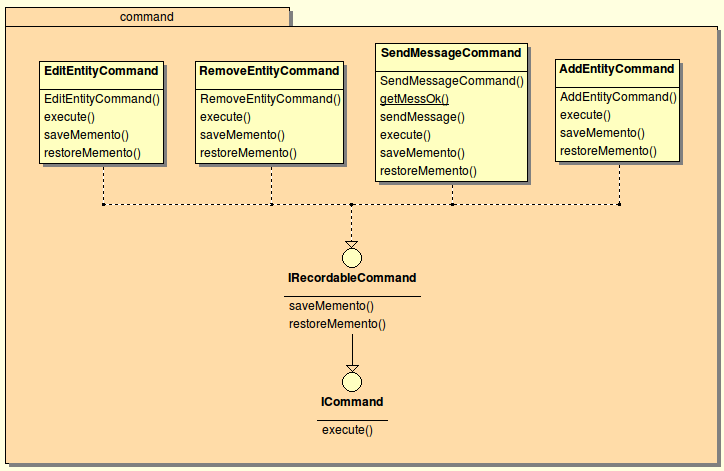
\includegraphics[height=280pt]{doc_dev-fig006.png}
\caption{Diagramme du patern command classique permettant de réifier les actions “client/serveur” possibles au sein de l’application.}
\end{center}
\end{figure}

\newpage
\subsubsection{Package handler}
\begin{figure}[htbp]
\begin{center}
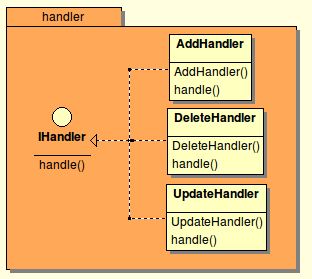
\includegraphics[width=233pt, height=209pt]{doc_dev-fig007.png}
\caption{Diagramme de classe du package handler.}
\end{center}
\end{figure}

Les \textbf{Handler} prennent des \textbf{IEntity} (côté client donc) et se chargent d’effectuer les modifications nécessaires pour mettre à jour la liste d’entités côté client et côté serveur.

Ils vont par exemple se charger de supprimer un véhicule côté client et donc d’envoyer le message de suppression au serveur via la classe \textbf{AgetacClient} du model.

Le fait de passer dans un handler va automatiquement déclencher une mise à jour côté client de l’interface graphique, car l’état du moteur va changer en fonction de l’action à prendre en charge.

\newpage
\subsubsection{Package engine}
\begin{figure}[htbp]
\begin{center}
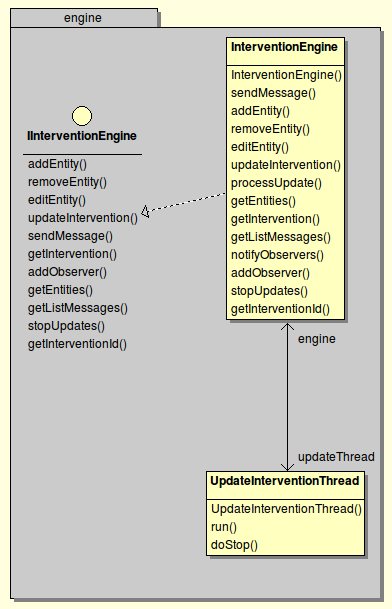
\includegraphics[width=293pt, height=456pt]{doc_dev-fig008.png}
\caption{Diagramme de classe du package engine.}
\end{center}
\end{figure}

Le moteur de l’application se charge de la connexion entre le client et le serveur. Il transmet les messages aux \textbf{Handler} en ce qui concerne les actions possibles (REST).

L’\textbf{UpdateInterventionThread} quant à lui, va se charger d’appeler la méthode \textbf{updateIntervention()} périodiquement (intervalle défini en dur dans le code du thread) afin de mettre à jour le client avec les informations récupérées sur le serveur.

Lorsque l’état du moteur change (donc quand sa liste d'entités est modifiée), il va notifier le contrôleur.
\newpage

\subsubsection{Package view}
\begin{figure}[htbp]
\begin{center}
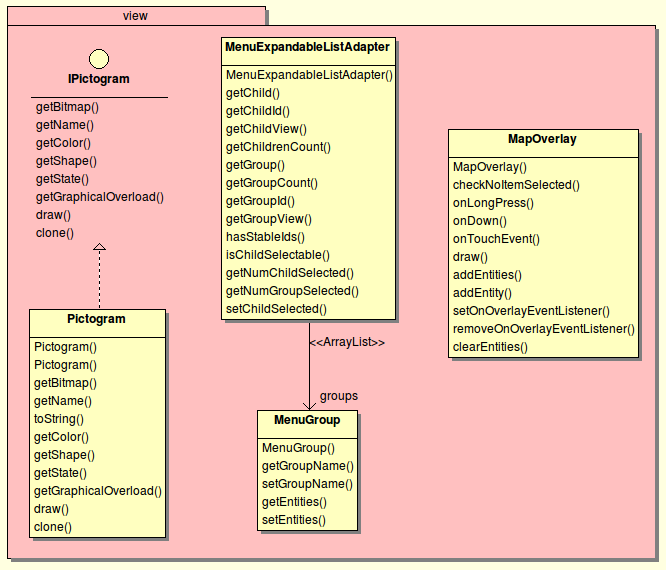
\includegraphics[width=499pt, height=427pt]{doc_dev-fig009.png}
\caption{Diagramme de classe du package view.}
\end{center}
\end{figure}


\textbf{MapOverlay} représente la carte de la SITAC. Il est capable de dessiner les différentes entités sur la carte et déclenche des évènements lorsque l’utilisateur interagi avec.

Le \textbf{MenuExpandableListAdapter} permet de dessiner les différentes entités dans le menu.

Un \textbf{Pictogram} est une image et est associé à une \textbf{Entity} et un \textbf{IModel}.

\newpage
\subsubsection{Package entity}
\begin{figure}[htbp]
\begin{center}
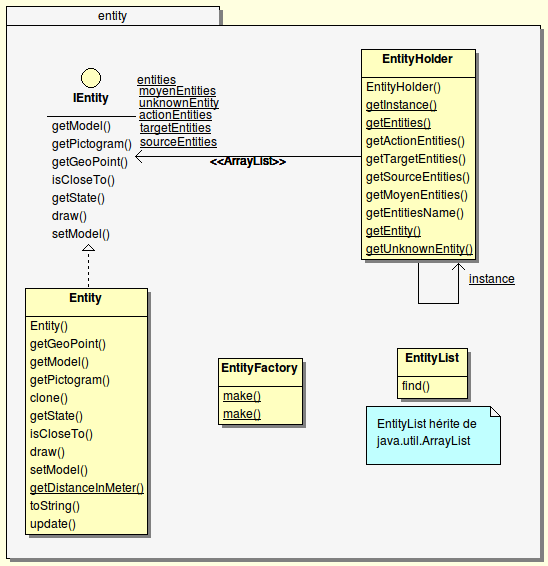
\includegraphics[width=410pt, height=424pt]{doc_dev-fig010.png}
\caption{Diagramme de classe du package entity}
\end{center}
\end{figure}

Les \textbf{IEntity} sont des objets qui contiennent un \textbf{IModel } et un \textbf{IPictogram.} Ils peuvent être dans différent états durant leur cycle de vie :

\begin{itemize}

\item[EntityState.MENU : ] une entité du menu, vide, qui sert de base ``clonable''.

\item[EntityState.ON\_SITAC : ] une entité avec un modèle bien défini et une position connue.

\item[EntityState.OFF\_SITAC : ] une entité avec un modèle bien défini mais une position inconnue (elle apparaîtra donc dans l'onglet ``Position à définir'' du menu).

\end{itemize}

\newpage
\subsection{Serveur}

\subsubsection{Diagramme de classe}

\begin{figure}[htbp]
\begin{center}
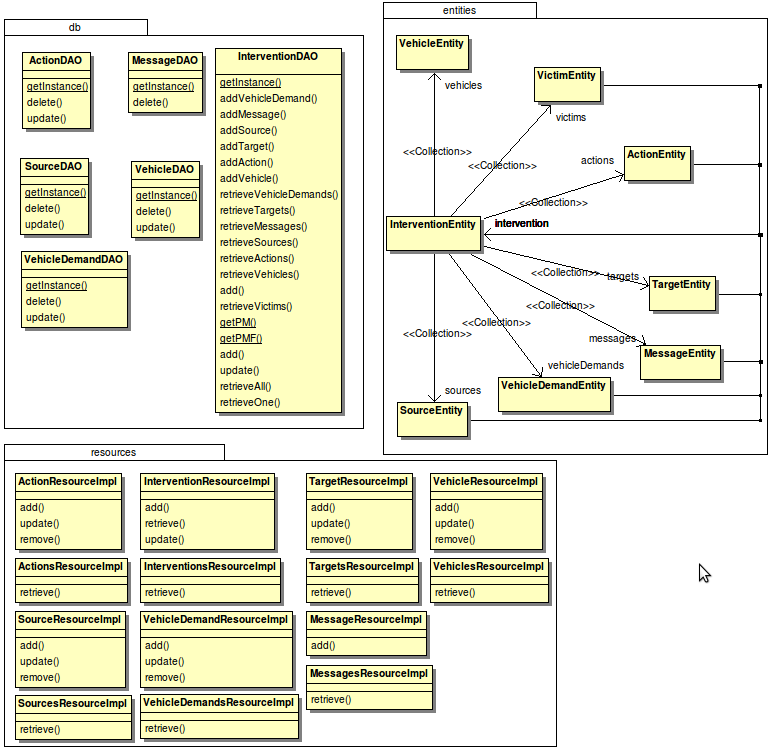
\includegraphics[width=460pt]{doc_dev-fig011.png}
\caption{Diagramme de classe du serveur}
\end{center}
\end{figure}

L'architecture du serveur est décomposée en une classe principale et quatre packages.
La classe « \textbf{Server.java} », qui se situe dans le package principal du serveur (\textbf{org.agetac.server}), a pour but d'initialiser le serveur et de lui associer un \textbf{Router}.\\


L'initialisation du serveur consiste en la création d'un \textbf{Restlet component} sur le protocole HTTP et le port 8888 auquel nous associons une \textbf{application}. L'intérêt des \textbf{Restlet components} réside dans le fait de pouvoir héberger plusieurs \textbf{applications} ayant des fonctionnalités très différentes, comme un client HTTP et un client SMTP, au sein d'une même JVM (Java Virtual Machine). Le but est de fournir une alternative portable, flexible et totalement orientée REST à l'API Servlet standard.\\


Une fois l'application créée, il faut lui associer un \textbf{Router}. Un \textbf{Router} est un objet Restlet permettant d'associer des URI à des ressources Restlet avec lesquelles la tablette cliente communiquera. Nous utilisons plusieurs templates d'URI :
\begin{itemize}
\item « /ressources » permet d'obtenir la liste de tous les objets du type ressource sur le serveur.
\item « /ressource/{ressourceId} »     permet d'obtenir un objet particulier du type ressource identifié par l'id ressourceId.
\end{itemize}
Ces deux templates d'URI sont combinés au sein du serveur sur chaque ressource pour obtenir par exemple la liste des objets de type ressource2 au sein d'un objet particulier de type ressource1 : « /ressource1/{ressource1Id}/ressources2 ».
Toutes les URI sont associées à des classes d'implémentation de ressources situées dans le package “resources”.



\subsubsection{Le package entity}

Chaque classe dans ce package est de la forme « \textbf{typeEntity.java} » et représente un type de base avec toutes les fonctions \textbf{get()} et \textbf{set()} associées : \textbf{InterventionEntity}, \textbf{MessageEntity}, etc… Ces classes sont annotées pour pouvoir être persistantes et ont pour unique but d'être stockées.\\


\subsubsection{Le package db}

Dans ce package, nous avons des classes qui implémentent le pattern DAO (Data Access Object). Un DAO typique fournit une interface qui définit son lien avec le monde extérieur. Ce lien prend la forme d’une série de données d’accès et de méthodes de mise à jour de données.\\


Nous définissons nos propres interfaces de DAO, ce qui comporte beaucoup d’avantages, dont un en particulier : nous pouvons maintenant fournir une implémentation utilisant DataNucleus et JDO (dans le paragraphe suivant, nous expliquons brièvement ce qu’est JDO). Nous pouvons, en principe, fournir une implémentation DAO de cette interface utilisant JDBC par exemple ou utilisant n’importe quelle autre technologie persistante. Cela démontre une stratégie de conception souple permettant aux composants d’être échangés à un moment ultérieure.\\


Comme mentionné dans le paragraphe précédent, dans le serveur Agetac, nous utilisons JDO (Java Data Objects) pour la persistance : il s’agit d’une interface standard pour stocker des objets contenant des données dans une base de données. La norme définit des interfaces pour annoter des objets Java, récupérer ces objets via des requêtes et interagir avec la base de données en utilisant des transactions.\\


Une application qui utilise JDO peut travailler avec différents types de bases de données sans utiliser un code spécifique à une base de données (incluant les bases de données relationnelles, les bases de données hiérarchiques et les bases de données d’objets). Le serveur Agetac utilise une simple base de données, HSSQL, mais, comme pour les autres interfaces standards, JDO simplifie le portage de l’application vers d’autres solutions de stockage.\\


La procédure standard pour implémenter des méthodes DAO utilisant JDO est d’utiliser un PersistenceManager, obtenir une transaction et effectuer les opérations à faire (création, récupération, suppression, mise à jour). Compte tenu de la taille limitée de ce dossier, nous ne détaillerons pas plus ces étapes.\\


\subsubsection{Optimisation des classes de données}

JDO utilise une étape d’optimisation post-compilation dans le processus de construction du projet pour associer les classes de données avec l’implémentation JDO. Ici, le plugin Datanucleus pour Eclipse réalise cette étape automatiquement à la construction, mais tout le monde ne peut pas utiliser cette approche car elle requière des droits administratifs pour l’installer, ou une installation locale d’Eclipse. De notre côté, nous avons créé un script ANT qui effectue cette optimisation (DataNucleus fournit une tâche Ant pour améliorer les fichiers).\\


\subsubsection{Fetch groups}

Un autre chose à noter est l’utilisation de “Fetch groups”. Quand le client Android récupère une intervention, il ne demande pas seulement les champs primitifs de l’intervention (id, name), il veut aussi les véhicules, messages, sources, et autres éléments associés. En conséquence, quand nous récupérons une intervention dans la base de donnée, nous devons aussi récupérer les entités liées. Nous définissons ces entités pour correspondre avec l’utilisation des “Fetch groups”. Dans notre projet, ces groupes sont indiqués par des annotations Java.\\


\subsubsection{Mises à jour problématiques}

Un moyen de mettre à jour un objet avec JDO est de récupérer cet objet puis le modifier pendant que le PersistenceManager qui retourne cet objet est toujours ouvert. Les changements sont conservés quand le PersistenceManager est refermé. Cependant, dans le cas d’une application client/serveur, cela ne fonctionne pas.\\


Typiquement, dans un système client/serveur, on retire l’objet, on l’envoie au client pour traitement, puis le client le retourne au serveur qui est supposé appliquer ces changement. Au moment où l’objet est retourné au serveur pour enregistrer les changements, le PersistenceManager qui a initialement récupéré l’objet n’existe plus.\\


Pour atténuer ce problème, quand le serveur est appelé à mettre à jour un objet, nous recherchons cet objet dans la base de données et, s’il est trouvé, nous associons (en utilisant la librairie ModelMapper) les champs de l’objet envoyé aux champs de l’objet retiré.\\


\subsubsection{Le package resources}

Ce package contient deux classes par type de ressource : une classe permettant de travailler sur une instance particulière de la ressource, « \textbf{typeResourceImpl.java} », et une classe permettant de travailler sur la liste de toutes les instances de cette ressource, « \textbf{typesResourceImpl.java} ».\\


Chaque classe étend ServerResource de l'API Restlet et implémente son interface contenue dans le Model, « typeResource » ou « typesResources ». Ces classes implémentent les fonctions add(), remove() et update() permettant d'ajouter, de supprimer ou de mettre à jour la ressource. Ces fonctions prennent en entrée un objet \textbf{typeDTO} (Data Transfer Object) envoyé par les tablettes clientes et mettent à jour la persistance.\\


\subsubsection{Le package client}

Il s'agit d'une IHM (Interface Homme Machine) permettant d'interagir directement avec les informations contenues sur le serveur. Ce package est articulé autour de trois sous-packages, « controller », « model » et « view » permettant de décomposer cette IHM selon le pattern MVC (Modèle Vue Contrôleur).\\

Le pattern MVC est un pattern qui organise la conception d'une IHM : le modèle gère ou décrit les données, la vue correspond à l'interface directe avec laquelle l'utilisateur interagit et le contrôleur prend en charge la synchronisation et la mise à jour du modèle et de la vue.\\

\section{Fonctionnement}


\begin{figure}[htbp]
\begin{center}
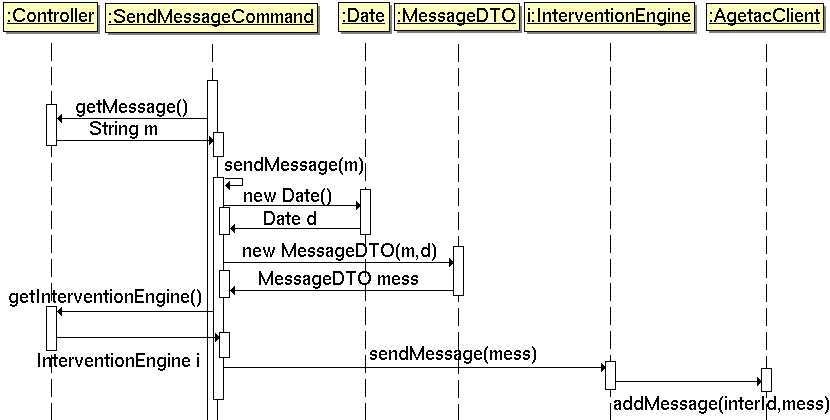
\includegraphics[width=460pt]{doc_dev-fig012.png}
\caption{Envoi message côté client.}
\end{center}
\end{figure}

\begin{figure}[htbp]
\begin{center}
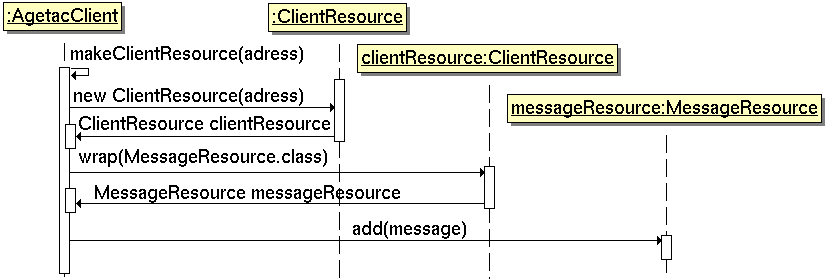
\includegraphics[width=460pt]{doc_dev-fig013.png}
\caption{Envoi message côté Model.}
\end{center}
\end{figure}

\begin{figure}[htbp]
\begin{center}
\includegraphics[width=460pt]{messserv.png}
\caption{Envoi message côté serveur.}
\end{center}
\end{figure}

\end{document}
